\part{Conclusion and Perspectives}
%\setcounter{chapter}{0}

~\vspace{1cm}
\begin{flushright}
{\it The law of unintended consequences pushes us ceaselessly through the years, permitting no pause for perspective.}\\
Richard Schickel
\end{flushright}
\vspace{2cm}

This last part wraps up the thesis. The first chapter summarizes by going back over the context and requirements, recalls the contribution and emphasizes its adequateness in relation to the requirements. After which, a short section discusses the benefits and limitations identified in this thesis.\\
The second chapter of this part shapes some perspectives of scientific development for this contribution, while the last chapter presents industrial perspectives. 

\chapter{Conclusion}

This chapter globally summarizes the work carried out for this thesis. Starting from the requirements, this chapter goes through the contribution, discusses its appropriateness to the context and ends by highlighting some benefits and drawbacks.

\section{Reminder of Context}

The ageing of the European population prompted the community to search for solutions to support this evolution. In this context, several issues have to be addressed in parallel. Firstly, the domain of health care suffers from a manpower shortage that could result in a decrease in the health service quality. Secondly, places in health care centers are not indefinitely extensive and centers will shortly reach their maximum capacities. Finally, a day spent in health care centers, or hospitals, is quite expensive and funding is limited.\\
Several projects have been started to try to address these issues. The Ambient Assisted Living (AAL) joint program has been created to promote such projects and emphasize the interest of Europe in advances in this domain. The {\it Innovation Domicile Autonomie (IDA)} project, initiated by the City of Rennes and the Greater Rennes Area, fits into this scheme with an evaluation of how the use of Information and Communication Technologies (ICT) can help to cope with these problems.\\
After a precise assessment of elderly people's needs, this project measured the adequateness of several industrial solutions to help and support elderly people at home. Among others, home automation technologies have been analyzed to work out their possible contribution to this problem. Rapidly, the survey demonstrated that a unique solution cannot be applied in all cases. Each person has different needs and requirements, which implies that the solutions need to be adapted for each deployment. Also, manufacturers reach their limits when a device has to be specialized for each user.\\

The technical solutions designed in this context require some software systems to bridge the gap between mass market home automation devices and customized solutions. To meet certain needs, these software systems must cope with several requirements.

\section{Summary of requirements}
\label{sec:concluRequirements}

{\bf Interoperability} is the first requirement software systems have to cope with. Indeed, solutions proposed to improve elderly people's comfort at home may be composed of multiple products, from different manufacturers. Each device taking part in a solution addresses a particular need of the person and makes the solution closer to the ideal one. In any case, elements of the solution have to communicate with each other to render a global service, but the diversity of manufacturers makes the interoperability of devices a real problem.\\
The definition of a common communication interface for all components of the system could solve the problem, but it requires that all devices are re-engineered to implement this communication interface. With this approach, all products already available cannot be used, because they will never implement this interface. Since the solution must not be limited in terms of usable products, it avoids the definition of a global communication interface.\\

{\bf Adaptation and Evolution} are the two main concerns to deal with in this domain. Software systems dealing with objects or services linked to actions of everyday life, have to take into account the environment in which they are being executed. They should be able to dynamically adapt to changes while running, in order to maintain a level of services, or functionalities. These adaptations should not require any restart of the system, since it would disable all functionalities for the time of restart. This is a real problem considering the trasmission of a request for assistance.\\
Needs, uses, protocols and technologies are changing. Some functionalities may finally be required, whereas others can become useless and need to be uninstalled. Security or communication protocols can be improved and deployed in new versions that have to be taken into account without needing to re-implement the entire system. Software systems must be ready to accept future and unforeseen evolutions, such as the installation of new services/functionalities.\\

{\bf Openness and Remote Control} are intended to make all functionalities of the software system available for third party applications. Indeed, the connection of some products may require that the system is accessible through a specific application protocol. This availability offers means to connect to the system with no need to be aware of its internal organization. The only interest is on using the functionalities or devices. It is an open door for new unforeseen appliances and for external contributions. Each one can take part in adding a smart behavior on top of a reliable set of functionalities.\\
Remote control may be required for a carer to remotely check if everything is doing well. It may also help in supporting remote-assisted management of the home for instance, or to remotely deploy new appliances or maintain the system.\\

{\bf Variability Management and Distribution} issues are linked to the need for customization of solutions, and to the dispersion of deployments. Since solutions for elderly people have to be customized to best fit their needs, the set of options of the system may become barely manageable. Some deployments may require high computation power, whereas others may run on tiny execution platforms. Moreover, evolutions of services or protocols may not be applied to all running systems at the same time, making the management of versions even more complex. All these elements lead to a huge number of configurations and to complex variability management.\\
Software systems have to be aware of these problems and offer tools in order to help system designers and technicians. Decision-helping tools should be created to support the design of software systems based on requirements and available devices.\\

{\bf Safety \& Security} is a very important concern for home automation systems. It is even more important when the system is aimed at improving the quality of life of dependent people. A minimum service level has to be guaranteed, for inhabitants not to remain stuck in the house in the case of an emergency for instance. Moreover, access to the system has to be secured to disallow anonymous control, but not tedious for authorized people in a normal use case.\\

{\bf Acceptability \& Accessibility} are issues that must be addressed, particularly when a software system takes responsibility for part of the home management. The \gls{aal} domain is a complex environment in which solutions must support the activity of elderly people and help carers in their work. For both of them, the system must not be perceived as a new constraint, or considered as stigmatizing. People must accept the solution deployed in their home and have to be reassured that they will keep a hand on things that could happen.\\


\section{Survey of existing approaches}

Among all the requirements listed in section~\ref{sec:concluRequirements}, the survey of existing approaches concentrated on interoperability, adaptation, evolution, openness and variability management.\\

Scientific literature abounds with proposals using different approaches to cope with interoperability, adaptation or remote control concerns in several applications. Generally, service-based propositions~\cite{OSGI:r4,ESB} sound helpful in targeting the interoperability of devices, but clearly lack description of the running application once deployed. They also bring essential ideas to properly handle the sporadic appearance of elements, since a service can be started and stopped at any time.\\
Component-based architectures~\cite{Georgiadis:2002,RobVanOmmering:2000,Bruneton:2006} provide an ideal abstraction level to meet the requirements for a virtual representation of home automation devices. However, components' ports are often defined by an API. This strict definition may disallow some connection unforeseen at design time, without the help of {\it ad-hoc} connectors.\\
Using components for SOA~\cite{sca:specs,Melisson:2010,Escoffier:2007} is certainly the best approach for our concerns, since the benefits of the first balance out the drawbacks of the second.\\
Transversally to any approach, model-driven engineering methods and techniques come with a lot of tools for virtual element manipulations. They seem handy for runtime management of devices, for the description of software systems, and for variability management.\\

All the approaches, tools, and frameworks considered in this survey have been reported in table~\ref{tab:adequatness}. This table synthesizes the strengths and weaknesses of each approach in relation to the requirements identified.






\section{Outline of the contribution}


Inspired by achievements in electronics this thesis contributes to improving the flexibility of software systems, while maintaining a high level of reliability. The contribution is threefold.
\par (1) A new component model, which improves flexibility to enable the connection of heterogenous components.
\par (2) Tools from model-driven engineering, to create, edit, simulate and validate the structure and behavior of component assemblies, prior to their (re-)deployment. 
\par (3) A runtime environment built on top of a service-based architecture, to support evolutions, adaptations and openness required by the proposed component model.\\

The implementation of this contribution called \enti{} is composed of several elements. Each of them, presented as a layer, addresses a particular concern of the global problem.\\

{\bf Device Interoperability} takes responsibility for the communication with real devices and between their virtual representatives in the {\it Component Model} layer. A mix of drivers (to connect the real to the virtual world), and asynchronous message-based communications, enables the connection of components previously marked as not compatible.\\

The {\bf Component Model} layer brings up the necessary structures and methods to handle the virtual representation of real devices. It provides a unified description of possible actions and available information, using the paradigm of ports. In this model, ports can be of two kinds: synchronous (service ports) or asynchronous (message ports). This component model helps to provide a detailed view of components, with precise information for the {\it Model@Runtime} layer to work properly. Tools have been made available to ensure the synchronization of models and implementation codes of components.\\

The {\bf Model@Runtime \& Checkers} layer involves necessary tools to ease the management of the system. Specificities of components' implementations are invisible at this level, thanks to the {\it Component Model} layer. Simulations and checks can be safely performed at this level of abstraction, with no consequences on the running application, since the model view is synchronized but independent from the execution. {\it Model@Runtime \& Checkers} contribute to enabling management of the system at runtime, to offering tools for checks and validations, to improving the safety of the solution, and help in dealing with the variability of the system.\\

The {\bf Wrappers} layer takes responsibility for publishing the devices present in the system, on application level networks. This ability opens our solution to existing and future protocols. Often too heavy to be embedded in basic devices, this layer makes all devices available on application level protocols for free.\\

{\bf Service-Oriented Runtime} comes to completes the contribution by providing an execution environment for the new component model. It brings life to the {\it Model@Runtime} by supporting dynamic {\it adaptations} and {\it evolutions} while running.\\


\section{Adequateness of the contribution}

The \gls{aal} context, the home automation domain description and the state of the art, led to an extraction of a list of requirements. These requirements have been stressed as the essential abilities a software system should be able to provide to be used in this context. The table~\ref{tab:adequatness} recalls the table presented in chapter~\ref{ch:summary}, in which all existing approaches were presented, and where their participation with relation to each identified concern had been reported.\\
The last line completes this table with \enti{}, and shows that it fits most of these requirements.\\
\begin{table}[h!]
\begin{tabular}{cm{.23\textwidth}|| >{\centering\arraybackslash}m{.06\textwidth}| >{\centering\arraybackslash}m{.07\textwidth}| >{\centering\arraybackslash}m{.09\textwidth}| >{\centering\arraybackslash}m{.08\textwidth}| >{\centering}m{.11\textwidth}| >{\centering\arraybackslash}m{.08\textwidth}|}
 & & {\tiny Interop.} & {\tiny Openness} & {\tiny Dynamic Adaptation} & {\tiny Static Evolution} & {\tiny Variability Management} & {\tiny Safety \& Security}\\
 \hline\hline
 \multirow{7}{7mm}{\begin{sideways}\parbox{25mm}{\small\centering Generic Approaches}\end{sideways}}
 %&{\small Hydra} 		& + & + & + &  &  & \# \\
 &{\small OSGi~\cite{OSGI:r4}}				&  & + & + & + &  &  \\ 
 &{\small ESB~\cite{Chappell:2004}}								& + & + &  & + &  &  \\
 \cline{2-8}%\hline
 %\multirow{3}{7mm}{\begin{sideways}\parbox{13mm}{\centering \tiny Component Models}\end{sideways}}
 &{\small Darwin~\cite{Georgiadis:2002}}		&  &  & + & + &   & + \\ 
 &{\small Koala~\cite{RobVanOmmering:2000}}	&  &  &   & + & + & + \\
 &{\small Fractal~\cite{Bruneton:2006}}		&  &  & + &   &   &  \\
 \cline{2-8}%\hline
 %\multirow{2}{7mm}{\begin{sideways}\parbox{12mm}{\centering \tiny Component Models for SOA}\end{sideways}}
 &{\small SCA~\cite{sca:specs}}				&   & + &  & + &  & +\\
 &{\small FraSCAti~\cite{Melisson:2010}}	 	& + & + & + & + &  & + \\
 &{\small iPOJO~\cite{Escoffier:2007}}		&  & + & + & + &  &  \\
 \hline\hline
 \multirow{9}{7mm}{\begin{sideways}\parbox{30mm}{\small\centering  Domain-Specific Approaches}\end{sideways}} 
 &{\small uMiddle~\cite{Nakazawa:2007}}		&  &  &  &  &  &  \\
 &{\small SOPRANO~\cite{Wolf:2010}}			&  &  & + & + &  &  \\
 &{\small Ga\"ia~\cite{Roman:2002}}			& + &  & + & + &  &  \\
 &{\small Dia Suite~\cite{CASSOU:2010}}		& + & + &  &  & + & + \\
 &{\small Habitation~\cite{Jimenez:2009}}	& + &  &  &  & + &  \\
 &{\small WADL~\cite{Cervantes:2008}}		& + &  & + & + &  &  \\
 &{\small PervML~\cite{Munoz:2006a}}			& + & + & + & + & + &  \\
 &{\small AutoHome~\cite{Bourcier:2011}}		&  & + & + & + &  &  \\
 &{\small WComp~\cite{Ferry:2011uq}}			& + &  & + & + &  & \\
 &{\small Niagara~\cite{Tridium:2008}}		& + & + &  &  &  &  \\
 \cline{2-8}
 &{\small EnTiMid} 							& + & + & + & + &  &  \\
 \hline
\end{tabular}
\caption{Adequateness of the contribution}
\label{tab:adequatness}
\end{table}

The Device Interoperability layer, helped by the Component Model, addresses the interoperability requirement. Openness is ensured by wrappers, for application level protocols, and by drivers for future manufacturers. Adaptation at runtime and evolutions are made available by the use of Model@Runtime techniques and the OSGi runtime for supporting the implementation of this contribution. Variability management is simplified by the presence of a model, but tools are still insufficient to properly cope with this issue. Finally, remote control is possible thanks to 1) the Model@Runtime for remote adaptations or evolutions, 2) the wrappers for remote application level control.

\section{Conservativeness}

During the state-of-the-art survey, some good properties were identified. The contribution of this thesis is moderate in relation to these properties.\\

The {\bf Reflexive Model} proposed by \gls{mde} is still available. The Model@Runtime layer is responsible for this ability and keeps an explicit and independent model reflecting the architecture living at runtime synchronized. This model allows for the creation of reasoners, able to perform changes on the model, with no immediate impact on the running system, until the model reaches conformity.\\

{\bf Externalized coupling} is provided by the Model@Runtime by enforcing the elicitation of links between components. Moreover, the presence of drivers imposes the components to be created with no idea about their usage. This externalized coupling makes it possible for reasoners to dynamically change component connections, and even components directly. The enforcement of the component independence requirement, to allow interoperability, also takes part in ensuring the externalization from the component implementation.\\

{\bf Hot deployment} is natively supported by the OSGi runtime execution environment used for \enti{}. Indeed, for reasoners to be able to adapt the system with new components, or for evolutions to be easily deployed, \enti{} had to preserve this property in the final solution.\\

{\bf Close Isolation enforcement} is imposed by the device interoperability layer and the entire \enti{} system. Types and instances are handled separately and all instances have independent life cycles since real devices can evolve independently.\\

{\bf Openness} was identified as a good property, but also as a key requirement, which has been addressed in this contribution, and explained in the validation.


\section{Immediate benefits}

\subsection{Development of components made easier}
The tools coming with this contribution aims at supporting the development of components. The component model forces developers to respect properties such as close isolation, or externalization of component couplings and makes the maintenance and the evolutions easier. The use of annotations in the component code and the availability of a code generator also simplify the everyday work of component developers. The code generator and the synchronization mechanism bring significant gains in terms of prevention of errors, time consumption and shorten the time elapsed from a new requirement to the solution.

\subsection{Simple creation of applications}
Thanks to the component model and modeling tools, the creation of applications is made very simple. Libraries of components can be imported into editors and components are assembled and connected using drag-and-drop interactions. If checkers so authorize, connections from port to port make it possible to connect any port to any other, whatever their roles or actions.\\
Designers of home automation devices are already familiar with this way of connecting things, since the model is very close to that of the electronic components. The design of a solution customized to meet a person's specific needs is thus quite quick and simple for engineers and technicians.

\subsection{Sustainability and precision}
The adaptation and evolution abilities of \enti{} improve the sustainability of deployed solutions. Present by default in the system, they offer the support for the evolution of both technologies and elderly people's pathologies, with no need to change the entire system. This way, a software system created to meet specific needs at a time, can be changed with a very limited cost, which makes the solution always precise and sustainable.

\subsection{Seamless integration of IoT and IoS}
The new component model enables the connection of heterogeneous components not designed to be working together. The heterogeneity can be due to the difference of manufacturer, protocol used, or media used, but can also be due to the object they represent. Several services available through the Internet have been wrapped into components, to enable the application to access a service such as an on-line calendar, a weather service, a picture-sharing service and even a famous social networking service. The component model enables seamless connection of a Google Calendar from the Internet to a light component for instance. The effect of such a connection could be to switch off the light when no appointments are specified.


\section{Limitations identified}

\subsection{Behavioral description}

The component model eases the structural description of a software system when people are very familiar with the description of its behavior. In addition to the component model (thus the structural description), it would be helpful to have a second tool to check and describe the behavior of the system. In this condition, an end user could be able to change the behavior of the system, without dealing with the structural description.\\
If the answer has not been provided yet, it may be because the problem is not simple once the behavior of the system can be described in several pieces. Indeed, thinking in a functional way makes people define how the system must behave when the door opens, or when an alarm is triggered, but with no consideration about the consequences on its global behavior. Moreover, the structural and the behavioral descriptions have interactions with each other.\\
Lastly, as non-experts of the domain, the description people can make of how the system must behave never takes errors or failures into account. From a linear description, erroneous paths have to be guessed and tested~\cite{Offutt:1997}.

\subsection{Port parameters}
Classical component models have been excluded in this thesis, because of the too strict specification of ports, making it impossible to connect two ports if their APIs are not aligned. But the problem of alignment has not completely disappeared in our component model. It has been moved from the implementation to the virtual representative of each component. Thus, the alignment of parameters passed through the ports has to be resolved at model level, before deployment.\\
Although this problem has not been addressed in this thesis, it has already been identified and scientists have already proposed some solutions under terms such as component connectors, which can have complex behaviors (cf Beugnard et al. in~\cite{Matougui:2005}). Mechanisms such as renaming or mappings~\cite{Clavreul:2010} of parameters could be implemented to cope with this issue.

\subsection{Too weak checkers}

Our experimentations did not require complex checks on models. Only simple structural checks, such as cycle detections, were implemented and used. Many checkers had not been completed since they were related to the business targeted. In the case of real deployments, they have to be completed to verify that no configuration marked as failing is asked for deployment.\\
Used at different steps, the checkers are different and they address various aspects of the application. Thus, the information, required to be able to perform each check properly, depends on what has to been checked. Since no  complete checker had been implemented, the information currently available in the model could be too poor for checkers to work.

\subsection{Variability management}

Variability issues have not been completely addressed, since a small set of components is sufficient for testing. Also, the number of components in the \gls{ida} experimentation was small enough to be handled manually. In the perspective of real deployments, the variations of configuration will impose the creation of tools to help in facing this huge variability.

\subsection{Improvements for embedded platforms}

In the context of the \gls{ida} project, the choice has been made to deploy \enti{} on a touch screen PC. This PC has high computational power and lots of memory compared to some more embedded platforms. But the deployment of a touch screen PC may not be necessary in all cases and some more embedded devices may be sufficient to automate some tasks. In any case, the runtime of \enti{} requires that a Java virtual machine is deployed on the platform first and thus providing enough power for the JVM to run.


\section{Contribution to the S-Cube NoE}

\subsection{The S-Cube Network of Excellence}

\begin{wrapfigure}{r}{.3\textwidth}
	\vspace{-1.4cm}
  \centering
  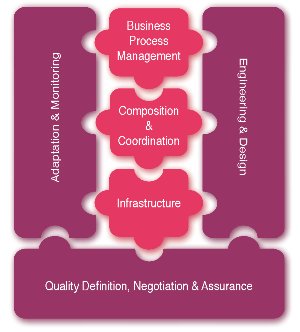
\includegraphics[width=.3\textwidth]{part1/pics/scube-overview.png}
  \caption{S-Cube Research Framework}
  \label{fig:scube-overview2}
  \vspace{-1cm}  
\end{wrapfigure}
S-Cube~\footnote{http://www.s-cube-network.eu/} is a European Network of Excellence (NoE) in Software, Services and Systems (S\up{3}). This NoE aims at making European research the leader in the software-services revolution. By connecting research to industry, and unifying multidisciplinary researches, S-Cube aims to develop agile and holistic service engineering methods, and to specify principles and techniques of service adaptation.\\
This European NoE has been funded by the European FP7 'Coordination' Research Programme  under the ICT theme. Along with strong collaboration and mobility opportunities beyond European research centers, S-Cube has funded several PhD theses in different layers of the S-Cube "BigPicture" (fig.~\ref{fig:scube-overview2}).\\

The skills of excellence of the INRIA Triskell team in which this theses was conducted, are dedicated to ease, and improve, software development methods, by the use of components, services, models and validations. Thanks to this team orientation, Triskell is involved in the S-Cube NoE, which has brought funding for two PhD theses. The research leading to the results presented in this theses has received credits from the European Community’s Seventh Framework Programme FP7/2007-2013 under grant agreement 215483 (S-Cube).\\

\subsection{Contribution}

The contribution of this thesis is aligned with the Work Package 1.2 : {\it Adaptation and Monitoring Principles, Techniques and Methodologies for Service-based Systems} of the Joint Research Activity(JRA) 1 : {\it Engineering and Adaptation Methodologies for Service-based Systems}\\

The general objective of the JRA-1, is to "devise an integrated set of principles, techniques and methodologies for engineering, adapting and monitoring hybrid service-based applications, while guaranteeing end-to-end quality provision and SLA conformance", according to the S-Cube description of work\footnote{DoW Amendment 4, December 6th, 2010}.\\
This thesis provides a new component model that: implies new engineering techniques and methodology, enables the adaptation of hybrid service-based application and offers means to perform checks and verifications to ensure the quality of services.\\

More precisely, the contribution of this thesis takes part in the JRA-1.2 work package, which aims to define novel principles and techniques for cross-layer monitoring and adaptation of Service-based Applications. If \enti{} does not address monitoring issues, it actually copes with adaptation requirements.\\

From the S-Cube perspective, \enti{} can be considered for handling adaptations of the infrastructure, or of the composition and coordination layer (see figure~\ref{fig:scube-overview}). Coupled with other layers, it can take part in the cross-layer adaptation mechanism.






\chapter{Perspectives}
\section{In research}

The contributions of this thesis leave some questions open, and have opened some doors. Therefore, the perspectives of this work aim at investigating and answering questions that have not been yet addressed, or go one step beyond into new uses of this contribution.


\subsection{IDA, second phase}
Conclusions from the experimentation led in the context of the \gls{ida} project shaped a promising future for the use of such tools, in the AAL domain. Even if the maturity of \enti{} and the objective of the first phase of the project did not allow testing of \enti{} in a real deployment situation, the protagonists (industrialists, carers, social workers and elderly people) have shown an interest in the provision of customized solutions for each person.\\
Currently, the second phase if the IDA project is being set up. Hopefully, it will be the moment for \enti{} to perform the last checks and to validate both the scalability and variability management, on real deployment.


\subsection{End User Programming}

End User Programming~\cite{Ko:2011} relates to the ability for anybody to program something. For instance, when a user programs the hours of start and stop of the heating system, he is actually programming. In the context of the IDA project and following the idea that inhabitants must be able to keep control of things in their homes, end user programming sounds like a very promising, but yet challenging perspective.\\

\subsubsection{Which description language ?}
Software developers like to be able to use the keyboard only. A graphical user interface, with drag-and-drop interactions to create assemblies, will probably not meet the requirements of this kind of population. For them, a textual language seems to be the simplest thing.\\
On the other hand, inhabitants do not all have skills in programming languages, and especially not elderly people. They would probably express their requirements for the behavior of the system in another way. The question is which one.\\

We had a range of description tools at our disposal, from a textual domain-specific language to a visual language composed of icons and boxes, linked with arrows. A solution for this problem probably lies somewhere in between these two extreme proposals and is surely not unique. Indeed, for the same system, an elderly person will probably be lost in a textual language and an engineer may be frustrated at being unable to express himself as usual.\\

The validity of the behavior described is also challenging. End users may not have a global vision of the system and thus may ask for a behavior that could lead the system to failure. Secondly, people naturally express the nominal behavior, without being concerned about possible deviations of this behavior. To address this problem, tools have to be proposed to check the validity of the nominal behavior and track and check any possible variation in the scenario.\\

The unique and universal language for describing how things have to behave will probably never exist. Because each user has a different kinship with technologies, systems should offer several edition tools, out of which the end user selects the handiest for him.


\subsubsection{Fuzzy Logic and Learning Algorithms}

In the hypothesis that people are able to describe a behavior of a function, how could they know about the limits of values? In other words, if a user is defining a behavior for the light, how could he know the minimum and maximum values that the light sensor can sense ?\\
The fuzzy logic paradigm~\cite{Chauvel:2008,Mendel:2001} proposes to use terms and non-fixed values in decision algorithms. Indeed, a fixed value is never appropriate because a regulation value must be modifiable. This paradigm makes it possible to work with terms and rough values only, because thresholds are computed at runtime. During the execution, users can act on these thresholds by telling the system about good or bad situations. Quite close to ideas of artificial intelligence, this approach could be coupled with some learning mechanisms, to go a bit further and re-simplify description of an application behavior.

\subsection{Distribution and Pervasiveness}

The distribution of applications brings several interesting facilities, such as load balancing, or redundancy to cope with failures of system elements. This question has not been properly addressed in this thesis, but may rapidly become a limitation. Moreover, working with devices brings \enti{} close to the ideas of pervasive computing. In this domain, objects' interactions are controlled by invisible nested software systems. Invisible for users, these systems have to self-reconfigure to take into account changes in their environments.\\

In the perspective of a large-scale deployment, distribution and pervasiveness can both come out as key requirements for some deployments. In \cite{Devescovi:2007}, Devescovi et al. propose algorithms for the self-organization of autonomic systems using the SelfLet approach. According to the presentation web page\footnote{http://selflet.sourceforge.net/}, a SelfLet is a "self-sufficient piece of software which is situated in some kind of logical or physical network, where it can interact and communicate with other SelfLets". This definition is very close to the definition of a smart device and SelfLets could be included in devices and device-controllers, such as firmware, to ease their integration.\\
This approach could foster the distribution of \enti{} on several nodes, help to prevent system failures, balance the load of resource-consuming components, or ease the connection of smart devices.


\subsection{Architecture Synthesis}
\label{sec:archiSynth}

The architecture synthesis goal is to assist in the creation of an application. Feature diagrams and automatic derivations into products, templates and wizards guiding the developer through the steps of product design, are two examples of tools enabling the synthesis of architectures.

\subsubsection{Dynamic Software Product Lines for the management of variability}

Not really addressed in the contribution, nor experimented in the validation, the management of variability in the domain of AAL and Home Automation is still a real problem. Luckily, the omnipresence of the model in all steps of the application-making process enables the use of well-known modeling tools to help in handling variability.\\

As proposed in~\cite{Morin:2010}, Aspect-Oriented Programming, coupled with Software Product Lines can be used to address this problem. Product Lines, a well-known variability management tool for supply chains, has been transposed into the software domain under the name of \gls{spl}. Large scale productions such as that of cars handles the variability of customers' requests using these product lines.\\
A product line consists of a base product that can be augmented with options selected by the customer. Software systems with a huge number of variable elements, such as component-based applications, can be defined the in the same way. The base functionalities of the software are described in the base product and specific options are plugged in according to the customer selection. The problem is that these tools have been set up to ease the one-shot creation of a product.\\

Dynamically-adaptive software systems are able to dynamically evolve after their creation, and \gls{spl}s are no longer sufficient to help in handling the description of things that can be changed at runtime. To cope with this issue, \gls{dspl} have been proposed. They enable the description of variation points during the execution of an application and make it possible to identify the exchangeable elements. The work carried out by Carlos Cetina et al. in this domain, presented in \cite{Cetina:2009}, is very close to what we want to achieve and reflects our future work.\\


\subsubsection{How can the behavior be descibed?}

In \enti{}, mapping components to leaf features in the \gls{dspl} makes it very simple to describe the desired configuration of the software at a high level of abstraction. Nevertheless, components in \enti{} are developed with a strong effort to respect the close entity principle and they do not know, or depend on each other. As a consequence, the \gls{dspl} can only support the description of the number of components, their types and the different options in the case of reconfiguration; in short, the structure of the assembly. Nowhere can the interactions between components be specified.\\

While still in its infancy, we proposed in~\cite{Istoan09a} an approach combining \gls{dspl} and Business Process Modeling. It enables the description of both architecture and behavior, by a combination of two modeling tools. Once coupled, these two models describe the structure of the application and its required behavior, which makes it possible to generate the entire system with connected components. As work in progress, this approach still has to be experimented in more depth.\\
Cassou et al. recently presented another approach to this problem of describing interactions. In \cite{Cassou:2011}, they introduce a "behavioral contract". These contracts are aimed at offering means to express the set of allowed interactions between components and describe both data and control-flow constraints. The integration of this idea with \enti{} may be studied in future work.


\subsection{Kevoree}

\enti{}, as an achievement of this thesis, has been highlighted as an interesting approach to address some identical issues in other domains.\\

For the principles of this contribution to be used in other contexts, \enti{} has recently been re-designed to become the customization of a more generic tool, specialized for home automation and AAL. Its name is Kevoree\footnote{http://kevoree.org}. The core mechanisms of adaptation, evolution, etc. have been moved into Kevoree in order to make them available for use cases other than home automation.\\

Whereas \enti{} is responsible for providing a set of services and components for Home Automation and AAL, Kevoree offers a set of tools for the component model. These include a framework to ease the implementation of components, a graphical editor to create component assemblies and a specialized runtime.\\
The development of Kevoree is actually part of the work in progress in the context of another thesis, which explores different improvements. For instance, questions about distribution and meanings of links between components.\\

{\bf Kermeta} is a \gls{dsl} optimized for metamodeling engineering. Developed in the TRISKELL team, it provides an integrated environment for Model-Driven engineering activities. Initially developed as a set of plugins for Eclipse, a work in progress is trying to make it run using the Kevoree tools.\\

{\bf Arduino} is an open-source electronics prototyping platform based on flexible, easy-to-use hardware and software. It is intended for artists, designers, hobbyists and anyone interested in creating interactive objects or environments, according to the manufacturer's web page. Recent developments shaped the idea of using Kevoree and the component model to ease sketches and the deployment of applications on Arduino platforms.


\subsection{Open Control/Command Operating System}

The component model of this contribution has been designed to allow for the connection of heterogeneous components. Inspired by electronics, the elements to be modeled and connected just need to be expressed in terms of components with inputs and outputs. Since almost all automated systems can be expressed this way, almost all systems can be modeled using the component model proposed in this contribution.\\
The independence of the model in relation to real devices-specificities enables the description of any application/system. Thus, \enti{} could take on the role of a universal control/command operating system, since the only difficult point is to develop the driver in charge of the interface between the real world and the component level. If a driver for an application can be created, \enti{} can help in controlling it.


\section{In industry}
\label{ch:industrialPerspectives}

The contribution of this thesis interests several audiences. The general public is curious to know about how computer science can help in improving elderly people's quality of life at home, since \enti{} was initially designed for the Ambient Assisted Living context. Everyone has or has had a family member who could have been helped by such a proposal. Industrialists are more interested in the good properties of the contribution. Since device manufacturers are familiar with electronic components, they easily understand how this component model works.\\
Starting from the validation scenario, in just 3 years a demonstration of \enti{} has been set up and presented in more than 10 public and scientific events. This demonstration stressed the adaptation aspect of the contribution in an AAL context.

\subsection{Public events}

Public events are an opportunity for the general public to discover what issues scientists are trying to resolve and how they do it. On the other hand, these meetings are also an opportunity for scientists to collect feedback on their work, from uninitiated persons. Uninitiated, in the sense that they are thinking about the problem for the first time. The questions asked are often very interesting, prompting you to step back from the details and to consider the proposal from a more global view.\\

The most important presentation was probably the science festival held in 2009 in Rennes, where \enti{} had been selected to represent the INRIA laboratory. The science festival, {\it Fêtes de la Science}\footnote{See the videos (in French) at http://videos.rennes.inria.fr/fete-sciences-2009/index.html} in French, is a national event lasting for 3 days. From Friday to Sunday inclusive, scientists present their everyday work, explain the problems solved, or the phenomenon involved in some experiments.

\begin{figure}
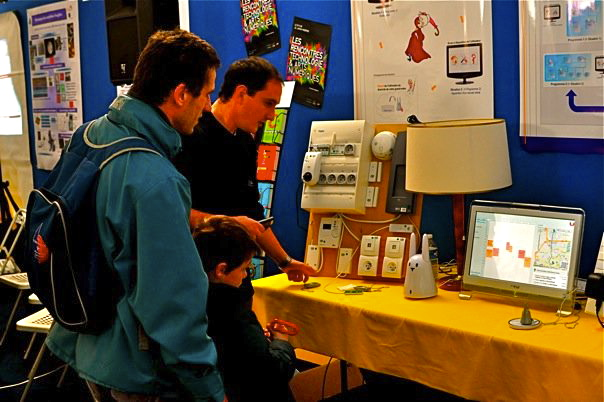
\includegraphics[width=\textwidth]{part4/pics/fdls.jpg}
\caption{Science festival presentation}
\end{figure}

During the first day, the festival admits only primary and middle school children. Visits are organized by groups and presenters have to explain their work to people aged from 7 to 15 years. This day is the most difficult day of the all festival. Not because the questions are complicated to answer, but because the explanation must be understood by everyone. This first day did not bring a lot of useful comments, or in any case, less than the two other days.\\

On Saturday and Sunday, the festival is open, for free, to families and anybody interested in sciences. These two days were a hard test for \enti{} and full of interesting discussions with people. Indeed, \enti{} had to run from 8am to 8pm without failure, disregarding touch-screen stress due to children's fingers, and in spite of the unpredicted use cases requested live by visitors.\\
It was the place for \enti{} to become enriched by new ideas, remarks, or people's experiences in facing elderly people's dependency problems. For the entire duration of the festival, no once did somebody say that \enti{} was useless, meaningless, or that the use case was not realistic. "It is not always that simple in real life" is the only remark we got.\\

Open days of the University of Rennes 1, or the opening celebration of the ESIR, the newly created engineering school of the University of Rennes 1, have also been two moments for exchanges with a large audience. Concerned by the studies, visitors' questions during these two events were more precise and more focused on what had been realized and how.\\
These demonstrations were sources of very interesting ideas to improve \enti{}.\\

Public presentations are very good opportunities to sense how the contribution exposed is perceived by anonymous people. None of them had a negative vision of the work, some had doubts and others asked about how to buy it. In my opinion it validates the utility of this contribution as perceived by people.\\

\enti{} has also been used as support for a demonstration called "{\it Leveraging Models From Design-time to Runtime. A Live Demo}" described in\cite{Morin09e}.

\subsection{Industrial perspectives}

The success of \enti{} has generated some industrial contacts. Several companies were interested in the abilities of this software to adapt and evolve at runtime. Most of them, close to the home automation domain, saw in \enti{} a great opportunity to enrich their products. But \enti{} was just a proof of concept, a prototype of research not ready to be deployed in the industry. This is partly the reason why \enti{} was not selected to be deployed in homes, in the IDA project.\\

Aware of this problem, a project of developing \enti{}, to make it ready for use in the industry had been submitted to the Regional Council of Brittany and accepted. This project funded the work of an engineer for one year, whose task was twofold. Firstly, to redevelop some parts of the contribution for it to be more stable, and secondly, to support the promotion of \enti{} in the industry. The development methods of \enti{} have been clarified and a second demonstration has been set up to focus more on the core functionalities and less on the home automation/AAL aspect.\\

In addition, a project of company creation is currently in progress and should end with the creation of a structure in charge of the promotion and support of \enti{} in the next few months. It was also a part of the development engineer's work to support the creation of this spin-off. 






